\section{Conceptos básicos}
\subsection{Teoría de colas}
\begin{figure}[H]
\centering
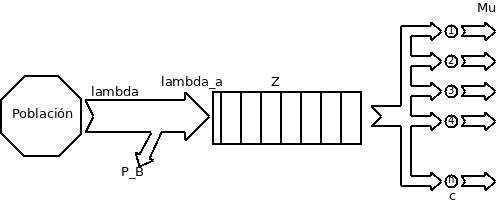
\includegraphics[width=0.9\textwidth]{Imagen/diateocolas.jpg}
\caption{Diagrama teoría de colas}
\label{dia:teocolas}
\end{figure}

\begin{itemize}
	\item $\mu$: Tasa de servicio, velocidad del sistema. Se mide en usuarios por unidad de tiempo.\\
	\item $\lambda$: Tasa de llegadas. Se mide en usuarios por unidad de tiempo.\\
	\item $\lambda_a$:Tasa de llegadas efectiva, la anterior menos los usarios expulsados del sistema. Se mide en usuarios por unidad de tiempo.\\
	\item c: Número de servidores del sistema.\\
	\item Z: Sistema de cola, lo más común \acrshort{FIFO}.\\
\end{itemize}
Para analizar el sistema siempre hay que asumir dos cosas: que el sistema no está colapsado y que se está produciendo un reparto uniforme entre todos los servidores.\\
\begin{equation}%[Tráfico ofrecido]
A_o=\frac{E(s)}{E(r)}=\frac{\lambda}{\mu}\text{ E=Tiempo/Tiempo}
\end{equation}
\begin{equation}%[Tráfico cursado]
A_c=A_0(1-P_B)=\frac{\lambda_a}{\mu}\text{ E=Tiempo/Tiempo}
\end{equation}
\begin{equation}%[factor de utilización]
\rho=\frac{A_c}{c}=\frac{\lambda_a}{\mu C}\text{ adimensional}
\end{equation}
\begin{example}
1 petición/hora se resuelve a 1 minuto/petición con una probabilidad de bloqueo 0. Calcula el factor de utilización para 1, 2 y 3 servidores:\\
\[A_o=A_c\]
\[A_o=\frac{\lambda}{\mu}=1\sfrac{pet}{h}1\sfrac{min}{pet}\sfrac{1h}{60min}=\sfrac{1}{60}E=16.7mE\]\\
\[\rho=\frac{A_c}{c}=
\begin{cases}
\sfrac{16.7}{1}=1.67\% & \text{para } c=1\\
\sfrac{16.7}{2}=0.83\% & \text{para } c=2\\
\sfrac{16.7}{3}=0.56\% & \text{para } c=3
\end{cases}\]
\end{example}

\subsubsection{Fórmulas de Little}
Las fórmulas de little son el resultado del análisis de las colas en régimen permanente.
\begin{itemize}
	\item $N(t)$: Número de usuarios en el sistema en un tiempo t.
	\item $N_s(t)$: Número de usuarios en los servidores en un tiempo t.
	\item $N_q(t)$: Número de usuarios en la cola en un tiempo t.
\end{itemize}
\begin{align}%[Fórmulas de little]
N=N_s+N_q\to L &=L_s+L_q\to W=W_s+W_q\\
L_x &=\gamma W_x\\
W_s=E(s)=\sfrac{1}{\mu} & \Leftrightarrow L_s=A_c\\
\gamma &=\lambda_a
\end{align}
\subsubsection{Distribución exponencial}
\begin{figure}[H]
\centering
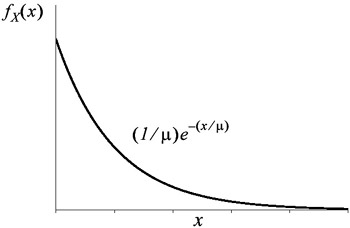
\includegraphics[width=0.9\textwidth]{Imagen/distribucionexponencial.jpg}
\caption{Distribución Exponencial}
\end{figure}
\begin{align}
P(t)=\mu e^{-\mu t} \leftarrow t\geq 0\\
Media=E(s)=\sfrac{1}{\mu}\\
P(t\leq T)=1-e^{-\mu T}
\end{align}
\subsubsection{Distribución de Poisson}
%%Insertar foto de la distribución de Poisson
\begin{figure}[H]
\centering
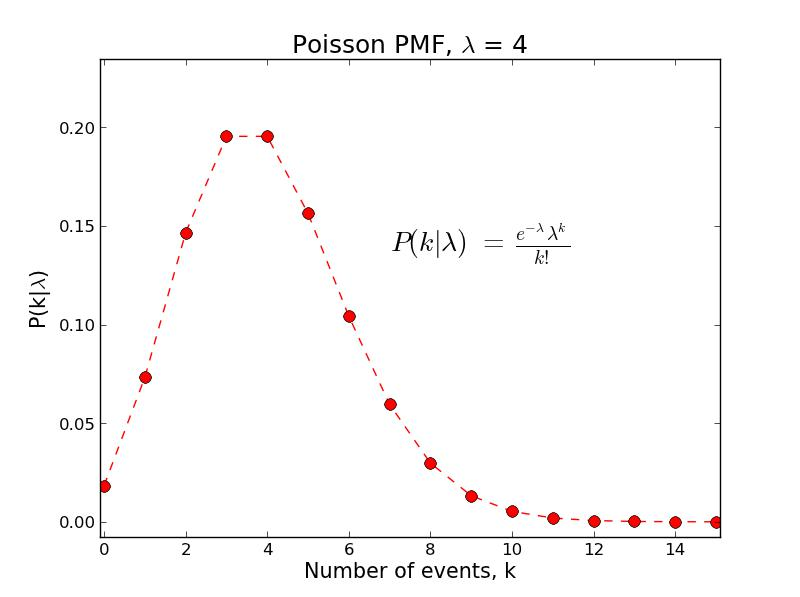
\includegraphics[width=0.9\textwidth]{Imagen/distribucionpoisson.jpg}
\caption{Distribución de Poisson}
\label{}
\end{figure}
\begin{equation}
P(k)=\frac{Ke^{-k}}{K!}
\end{equation}
\subsubsection{Nomenclatura teoría de colas}
\begin{center}
\framebox[1.1\width]{\huge{A/B/c/k/m/Z}} \par
\end{center}
\begin{itemize}
\item {A:} tiempo entre llegadas. m es la distribución normal(Poissoniana), i un modelo determinista y gi es el modelo general.
\item {B:} tasa de servicio. m es la distribución normal(Exponencial), i un modelo determinista y gi es el modelo general.
\item {c:} número de servidores.
\item {k:} capacidad del sistema. En caso de no venir especificado se asume capacidad "infinita".
\item {m:} tamaño de la población. En caso de no venir especificado se asume población "infinita".
\item {Z:} disciplina de la cola. En caso de no venir especificado se asume una cola \acrshort{FIFO}.
\end{itemize}
Cuando se habla de poblaciones o capacidades infinitas en realidad significa que el número es mucho mayor que el número de servidores. Población/Capacidad$>>$c.
\subsubsection{Modelo M/M/1}
Un modelo con llegadas poissonianas, tasa de servicio exponencial, 1 único servidor, una cola infinita, población infinita y una cola con disciplina \acrshort{FIFO}. Este modelo tiene una probabilidad de bloqueo nula $P_B=0$ con lo cual se cumple lo siguiente: $A_c=A_o=\sfrac{\lambda}{\mu}$. Al tener un solo servidor además se ve que $\rho=A_o$.
\begin{example}[M/M/1]
Tasa de llegadas 30$\sfrac{\text{clientes}}{\text{hora}}$ con una tasa de servicio de 115$\sfrac{\text{segundos}}{\text{cliente}}$ en un único servidor.
\[A_c=A_o=\frac{\lambda}{\mu}=30*115\sfrac{1}{3600}=0.9583E\] \\
\[\rho=A_c=A_0=0.9583=95.83\%\] Como se puede ver el servidor está a punto de saturarse.\\
\[L=\frac{\rho}{1-\rho}=23\text{ usuarios en el sistema de media}\]
\[L=\frac{\rho^2}{1-\rho}=22\text{ usuarios en la cola de media}\]
\[W=\frac{E(s)}{1-\rho}=45.96\text{ minutos en el sistema de media}\]
\[W=\frac{\rho E(s)}{1-\rho}=44.06\text{ minutos en la cola de media}\]
Los usuarios se quejarán. Hay que esperar 44 minutos en la cola para un servicio que tarda 2 en ser servido.
\end{example}
\subsubsection{Modelo M/M/c}
Un modelo con llegadas poissonianas, tasa de servicio exponencial, c servidores idénticos, una cola infinita, población infinita y una cola con disciplina \acrshort{FIFO}. Este modelo tiene una probabilidad de bloqueo nula $P_B=0$ con lo cual se cumple lo siguiente: $A_c=A_o=\sfrac{\lambda}{\mu}$.\\
\begin{example}[M/M/c]
Continuando el ejemplo anterior. $\lambda=30\sfrac{\text{clientes}}{\text{hora}}$ con una media de tiempo de servicio $\text{E(s)}=\sfrac{1}{\mu}=115\sfrac{\text{segundos}}{\text{cliente}}$. Contamos con 2 sevidores en lugar de uno. Compararlo con el anterior: W=46min $\text{W}_{\text{q}}$=44min\\
\begin{gather*}
A_o=\frac{\lambda}{\mu}=0.9583E=A_c\\
\rho=\frac{A_c}{c}=0.47915\simeq 48\% \\
L_q=\frac{\rho C(A_o,c)}{(1-\rho)}=0.28\text{ clientes en la cola de media}\\
W_q=\frac{E(s)C(A_o,c)}{c(1-\rho)}=34.2\text{ segundos en la cola de media}
\end{gather*}
Se puede ver una gran mejoría entre los 44 minutos con un único servidor y los 34 segundos en el caso de dos servidores.
\end{example}
\subsubsection{Modelo M/M/c/c}
Un modelo con llegadas poissonianas, tasa de servicio exponencial, c servidores idénticos, sin colas, población infinita y una cola con disciplina \acrshort{FIFO}. En este modelo es en el primero que vemos una probabilidad de bloqueo distinta de cero, $P_B=B(A_o,c)$ esta probabilidad se puede calcular gráficamente con las gráficas del Erlang B. En cambio aplicando esto a las fórmulas de little podemos ver lo siguiente: $L_q=0\to L=L_s=A_c=A_o(1-P_B)$\\
\begin{example}[M/M/c/c]
8 servidores con $E(s)=\sfrac{1}{\mu}=4\sfrac{\text{h}}{\text{usuario}}$ y una tasa de llegadas $\lambda=3\sfrac{\text{usuarios}}{\text{h}}$\\
\begin{gather*}
A_o=\frac{\lambda}{\mu}=12E\\
P_B=B(12,8)=42\%
\end{gather*}
\end{example}